\chapter{Heartbeat高可用集群}

Heartbeat提供了诸多集群基础架构服务,比如集群之间的消息传递、节点成员
身份、IP地址分配和迁移,以及服务的开启和停止。Heartbeat可以用来为
Apache、Samba和Squid等企业应用系统构建几乎任何一种高可用性的集群。此外,
它可以结合负载均衡软件使用,那样入站请求就可以由所有集群节点来分担。

本文中的示例集群将由2台运行Heartbeat的服务器组成。我们测试故障切换机
制的方法是,手动关闭服务器,检查它们服务的网站是不是仍然可用。下面是我
们的测试拓扑结构:

\begin{figure}[!htbp]
  \centering
  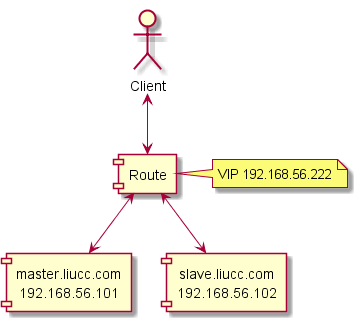
\includegraphics[width=0.5\textwidth]{img/heartbeat.png}
  \caption{heartbeat实验拓扑}
\end{figure}

映射服务所用的IP地址需要一直能够访问得到。通常,Heartbeat会为你将指定
的IP地址分配给主服务器上的虚拟网络接口卡。如果主服务器出现了故障,集群
会自动将IP地址切换到另一台可用服务器上的虚拟网卡。如果主服务器恢复正常
运行,它会再次将IP地址切换回到主服务器。由于具有迁移属性,这个IP地址被
称为“浮动”地址。

\section{安装Heartbeat}

在所有服务器上安装软件包

想组建集群,首先要使用yum,在每一个节点上安装必要的软件包:

\begin{verbatim}
yum install PyXML cluster-glue cluster-glue-libs resource-agents
\end{verbatim}

下一步,下载和安装官方CentOS软件库里面没有的两个Heartbeat RPM文件。

另外,你可以将EPEL软件库添加到源文件,并使用yum进行安装。

Heartbeat会管理Apache的httpd服务的开启和停止,所以停止Apache,并禁止它自动开启:

\begin{verbatim}
service httpd stop
chkconfig httpd off
\end{verbatim}

设置主机名称

现在设置服务器的主机名称,为此编辑每个系统上的/etc/sysconfig/network,并更改HOSTNAME这一行:

HOSTNAME=xxxxx.liucc.com 新的主机名称会在服务器下一次启动时激活。
你可以使用hostname命令立即激活它,不需要重启服务器:

hostname xxxxx.liucc.com 你可以在每一台服务器上运行uname -n,以此证实主机名称已正确设置好。

\section{配置Heartbeat}

想配置Heartbeat,首先要将其默认配置文件从/usr拷贝到/etc/ha.d/:

\begin{verbatim}
cp /usr/share/doc/heartbeat-3.0.4/authkeys /etc/ha.d/
cp /usr/share/doc/heartbeat-3.0.4/ha.cf /etc/ha.d/
cp /usr/share/doc/heartbeat-3.0.4/haresources /etc/ha.d/
\end{verbatim}

然后,你还得改动全部集群节点上的所有三个文件,以便与你的需求相匹配。

authkeys文件含有集群节点彼此联系时所使用的预共享密码。集群里面的每个
Heartbeat消息都含有该密码,节点只处理拥有正确密码的那些消息。Heartbeat
支持SHA1密码和MD5密码。在authkeys文件中,下列指令将验证方法设置为SHA1,
并且定义了所使用的密码:

\begin{verbatim}
auth 2
2 sha1 pre-shared-password
\end{verbatim}

保存该文件,然后使用命令

\begin{verbatim}
chmod 600 /etc/ha.d/authkeys
\end{verbatim}

为该文件授予只有root用户可以读写的权限。

下一步,在ha.cf文件中,定义计时器、集群节点、消息传递机制、第4层端口及其他设置:

\begin{verbatim}
## 日志##
logfile /var/log/ha-log
logfacility local0hea
## 计时器##
## 所有计时器设成以秒为单位。如果你需要以毫秒为单位设置时间,就使用‘ms’。##
## heartbeat间隔时间##
keepalive 2

## 超过这个时间后,节点被认为已停滞##
deadtime 15
## 一些服务器花更长的时间来启动。该计时器定义了证实服务器宕机之前所等待的额外时间。##
## 该计时器的建议时间是停滞计时器的至少一倍。##
initdead 120
## 消息传递参数##
udpport 694
bcast eth0
## 你还可以使用多播或单播##
## 节点定义##
## 确保主机名称符合uname -n ##
node master.liucc.com
node slave.liucc.com
\end{verbatim}

最后,文件haresources含有Heartbeat认为是主节点的那台服务器的主机名称,
另外还含有浮动IP地址。该文件在所有服务器上都一模一样,这点很重要。只要
主节点在正常运行,它就服务所有请求;Heartbeat停止其他所有节点上的高可
用性服务。Heartbeat检测到该主节点停机运行后,它会在集群中的下一个可用
节点上自动开启服务。主节点恢复正常运行后,Heartbeat会让它再次接手任务,
服务所有请求。最后,该文件含有负责高可用性服务的脚本的名称:这里是
httpd。其他可能出现的值有squid、smb、nmb或postfix,映射到通常位于
/etc/init.d/目录中的服务启动脚本的名称。

在haresources中,定义master.liucc.com.com为主服务器,定义
192.168.56.222为浮动IP地址,定义 httpd为高可用性服务。你不需要创建任何
接口,也不需要为任何接口手动分配浮动IP地址,Heartbeat为我们处理这项任
务:

\begin{verbatim}
master.liucc.com 192.168.56.222 httpd
\end{verbatim}

每一台服务器上的配置文件准备就绪后,开启Heartbeat服务,并将它添加到系
统启动项:

\begin{verbatim}
service heartebeat start
chkconfig heartbeat on
\end{verbatim}

这时,可以查看一下master节点上的IP地址信息,

\begin{verbatim}
[root@master ~]# ifconfig 
eth0      Link encap:Ethernet  HWaddr 08:00:27:4D:65:37  
          inet addr:192.168.56.101  Bcast:192.168.56.255  Mask:255.255.255.0
          inet6 addr: fe80::a00:27ff:fe4d:6537/64 Scope:Link
          UP BROADCAST RUNNING MULTICAST  MTU:1500  Metric:1
          RX packets:13825 errors:0 dropped:0 overruns:0 frame:0
          TX packets:10376 errors:0 dropped:0 overruns:0 carrier:0
          collisions:0 txqueuelen:1000 
          RX bytes:3095677 (2.9 MiB)  TX bytes:2253820 (2.1 MiB)

eth0:0    Link encap:Ethernet  HWaddr 08:00:27:4D:65:37  
          inet addr:192.168.56.222  Bcast:192.168.56.255  Mask:255.255.255.0
          UP BROADCAST RUNNING MULTICAST  MTU:1500  Metric:1

eth1      Link encap:Ethernet  HWaddr 08:00:27:BC:A6:E2  
          inet addr:192.168.56.201  Bcast:192.168.56.255  Mask:255.255.255.0
          inet6 addr: fe80::a00:27ff:febc:a6e2/64 Scope:Link
          UP BROADCAST RUNNING MULTICAST  MTU:1500  Metric:1
          RX packets:21609 errors:0 dropped:0 overruns:0 frame:0
          TX packets:61 errors:0 dropped:0 overruns:0 carrier:0
          collisions:0 txqueuelen:1000 
          RX bytes:4926438 (4.6 MiB)  TX bytes:6922 (6.7 KiB)

lo        Link encap:Local Loopback  
          inet addr:127.0.0.1  Mask:255.0.0.0
          inet6 addr: ::1/128 Scope:Host
          UP LOOPBACK RUNNING  MTU:16436  Metric:1
          RX packets:2696 errors:0 dropped:0 overruns:0 frame:0
          TX packets:2696 errors:0 dropped:0 overruns:0 carrier:0
          collisions:0 txqueuelen:0 
          RX bytes:5452373 (5.1 MiB)  TX bytes:5452373 (5.1 MiB)
\end{verbatim}

你可以借助命令tailf /var/log/ha-log,密切关注Heartbeat日志。

Heartbeat可用于多项服务。比如说,haresources中的下列指令将让Heartbeat
同时管理Apache服务和Samba服务:

master.liucc.com 192.168.56.222 httpd smb nmb 不过,除非你还在运行
Pacemaker之类的集群资源管理器(CRM),否则我不建议使用Heartbeat在单一
集群中提供多项服务。要是没有Pacemaker,Heartbeat使用IP地址监测第3层中
的集群节点。只要IP地址可以访问得到,Heartbeat无视服务在服务器节点上可
能遇到的任何崩溃或困难。

\section{测试}

一旦Heartbeat设置并运行起来,不妨对它测试一下。在所有三台服务器上创建
单独的index.html文件,那样你就能看清哪台服务器在服务页面。浏览到
192.168.56.222,如果你设置好了DNS,也可以浏览到相应域名。页面应该会从
master.liucc.com.com加载,你可以查看服务器1中的Apache日志文件来核实这一
点。试着刷新页面,证实该页面是否每次都从同一台服务器加载。

关闭主节点后,主节点产生的日志信息,

\begin{verbatim}
Apr 14 11:43:48 master.liucc.com heartbeat: [13928]: info: Heartbeat shutdown in progress. (13928)
Apr 14 11:43:48 master.liucc.com heartbeat: [14300]: info: Giving up all HA resources.
ResourceManager[14313]:	2015/04/14_11:43:48 info: Releasing resource group: master.liucc.com 192.168.56.222 httpd
ResourceManager[14313]:	2015/04/14_11:43:48 info: Running /etc/init.d/httpd  stop
ResourceManager[14313]:	2015/04/14_11:43:48 info: Running /etc/ha.d/resource.d/IPaddr 192.168.56.222 stop
IPaddr[14386]:	2015/04/14_11:43:48 INFO: ifconfig eth0:0 down
IPaddr[14372]:	2015/04/14_11:43:48 INFO:  Success
Apr 14 11:43:48 master.liucc.com heartbeat: [14300]: info: All HA resources relinquished.
Apr 14 11:43:49 master.liucc.com heartbeat: [13928]: WARN: 1 lost packet(s) for [slave.liucc.com] [36:38]
Apr 14 11:43:49 master.liucc.com heartbeat: [13928]: info: No pkts missing from slave.liucc.com!
Apr 14 11:43:50 master.liucc.com heartbeat: [13928]: info: killing HBFIFO process 13930 with signal 15
Apr 14 11:43:50 master.liucc.com heartbeat: [13928]: info: killing HBWRITE process 13931 with signal 15
Apr 14 11:43:50 master.liucc.com heartbeat: [13928]: info: killing HBREAD process 13932 with signal 15
Apr 14 11:43:50 master.liucc.com heartbeat: [13928]: info: Core process 13932 exited. 3 remaining
Apr 14 11:43:50 master.liucc.com heartbeat: [13928]: info: Core process 13931 exited. 2 remaining
Apr 14 11:43:50 master.liucc.com heartbeat: [13928]: info: Core process 13930 exited. 1 remaining
Apr 14 11:43:50 master.liucc.com heartbeat: [13928]: info: master.liucc.com Heartbeat shutdown complete.
\end{verbatim}

此时,备节点上的日志信息为:

\begin{verbatim}
ResourceManager[13103]:	2015/04/14_11:43:49 info: Acquiring resource group: master.liucc.com 192.168.56.222 httpd
IPaddr[13131]:	2015/04/14_11:43:49 INFO:  Resource is stopped
ResourceManager[13103]:	2015/04/14_11:43:49 info: Running /etc/ha.d/resource.d/IPaddr 192.168.56.222 start
IPaddr[13194]:	2015/04/14_11:43:49 INFO: Using calculated nic for 192.168.56.222: eth0
IPaddr[13194]:	2015/04/14_11:43:49 INFO: Using calculated netmask for 192.168.56.222: 255.255.255.0
IPaddr[13194]:	2015/04/14_11:43:49 INFO: eval ifconfig eth0:0 192.168.56.222 netmask 255.255.255.0 broadcast 192.168.56.255
IPaddr[13180]:	2015/04/14_11:43:49 INFO:  Success
ResourceManager[13103]:	2015/04/14_11:43:49 info: Running /etc/init.d/httpd  start
mach_down[13076]:	2015/04/14_11:43:49 info: /usr/share/heartbeat/mach_down: nice_failback: foreign resources acquired
mach_down[13076]:	2015/04/14_11:43:49 info: mach_down takeover complete for node master.liucc.com.
Apr 14 11:43:49 slave.liucc.com heartbeat: [12969]: info: mach_down takeover complete.
Apr 14 11:44:05 slave.liucc.com heartbeat: [12969]: WARN: node master.liucc.com: is dead
Apr 14 11:44:05 slave.liucc.com heartbeat: [12969]: info: Dead node master.liucc.com gave up resources.
Apr 14 11:44:05 slave.liucc.com heartbeat: [12969]: info: Link master.liucc.com:eth0 dead.
\end{verbatim}

如果这一切进展良好,测试一下故障切换机制:停止master.liucc.com上的
Heartbeat服务。浮动IP地址应该会迁移到服务器slave上,页面应该会从该服务
器加载。迅速看一下slave的Apache日志,应该可以证实这一点。如果我们重启
了服务器master上的heartbeat服务,浮动IP地址应该会按照haresources中的设
置,从活动节点迁移到服务器slave上。

当我们把master上的heartbeart重新运行起来,这时,观察slave节点的日志信息,

\begin{verbatim}
ResourceManager[13654]:	2015/04/14_13:52:20 info: Releasing resource group: master.liucc.com 192.168.56.222 httpd
ResourceManager[13654]:	2015/04/14_13:52:20 info: Running /etc/init.d/httpd  stop
ResourceManager[13654]:	2015/04/14_13:52:21 info: Running /etc/ha.d/resource.d/IPaddr 192.168.56.222 stop
IPaddr[13727]:	2015/04/14_13:52:21 INFO: ifconfig eth0:0 down
IPaddr[13713]:	2015/04/14_13:52:21 INFO:  Success
Apr 14 13:52:21 slave.liucc.com heartbeat: [13641]: info: foreign HA resource release completed (standby).
Apr 14 13:52:21 slave.liucc.com heartbeat: [12969]: info: Local standby process completed [foreign].
Apr 14 13:52:21 slave.liucc.com heartbeat: [12969]: WARN: 1 lost packet(s) for [master.liucc.com] [10:12]
Apr 14 13:52:21 slave.liucc.com heartbeat: [12969]: info: remote resource transition completed.
Apr 14 13:52:21 slave.liucc.com heartbeat: [12969]: info: No pkts missing from master.liucc.com!
Apr 14 13:52:21 slave.liucc.com heartbeat: [12969]: info: Other node completed standby takeover of foreign resources.
\end{verbatim}

正如我们所见,使用Heartbeat,在RHEL下组建一个高可用性的Apache集群是件
很容易的事。虽然我们使用了2台服务器,但Heartbeat在节点数量更多或更少
的环境下应该同样没问题。Heartbeat对节点数量没有任何限制,所以你可以根
据需要扩展所设置环境的规模。

